\section{Server}
Der Server zur Ansicht der Daten und Konfiguration der Anlage wird von dem ESP8266
Mikrocontroller bereitgestellt. Dieser verbindet sich mit dem heimischen Netzwerk.
Über die IP des ESP8266 kann man auf die Webseite zugreifen und bekommt die Graphen
zur Feuchtigkeit der Pflanzen sowie Einstellungsmöglichkeiten für beispielsweise Name
der Pflanze und gegossene Wassermenge angezeigt.

\subsection{Konfiguration}
Gestartet wird der Server durch $server.on(''/'', handleRoot);$ aus der Bibliothek \textit{ESP8266WebServer.h}. \textit{server} ist ein Objekt der ESP8266WebServer Klasse. Die Funktion teilt dem
Server mit, dass sobald sich ein Client auf den Root des Servers - also die IP-Adresse
des ESP8266 - verbindet, soll die Funktion \textit{handleRoot()} aufgerufen werden, die im Teil
Webseite (siehe \ref{handle}) erklärt wird.

Sollte ein User versuchen auf eine andere Seite als Root zugreifen wollen, wird die
Funktion \textit{handleNotFound()} aufgerufen. Dem User wird dann eine Error 404 Seite gezeigt,
die den versuchten Aufruf zeigt und dass dieser nicht gefunden werden konnte.

\subsection{Webseite}
Die Webseite für den User zeigt den Namen der jeweiligen Pflanzen an sowie Informationen
zur Feuchtigkeit und Einstellungsmöglichkeiten.
\begin{figure}[ht]
    \centering
    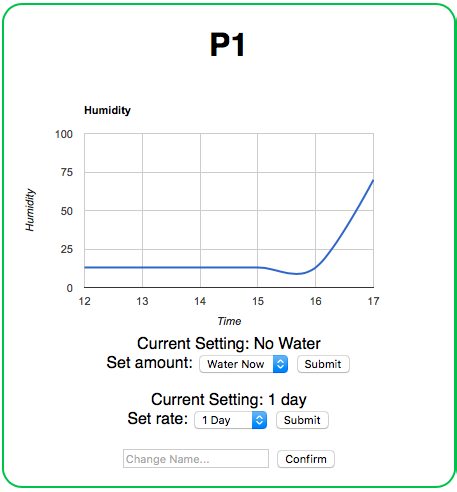
\includegraphics[width=0.7\textwidth]{images/seite2}
    \caption{Auszug der Webseite}
\end{figure}

\subsubsection{Graphen}
Die Graphen stellen den Wert der Feuchtigkeit aufgetragen über die Zeit dar. Die Daten
hierfür kommen direkt von den Sensoren des Arduino und werden vom ESP8266 in einem
Array gespeichert.
Das Array wird als DataTable an die Google Api weitergegeben. Von dort bekommt der User
den erstellten interaktiven Graphen übermittelt. Diese können durch Parameter wie Titel,
Kurventyp, Beschriftungen und Legenden verändert werden.
Dadurch, dass der Graph direkt an den User gesendet wird, entsteht auf dem ESP8266 keine
Last den Graphen zu erstellen oder zu speichern.

\subsubsection{Einstellbare Parameter}
Auf der Webseite befinden sich auch Parameter für jede Pflanze, die der User verändern kann.
Zur Personalisierung kann der angezeigte Name einer Pflanze geändert werden, beispielsweise
zur Art der zu überwachenden Pflanze. Dies geschieht über ein Textfeld, welches \textit{"Change Name..."}
anzeigt. Per Klick auf den \textit{"Confirm"} Button wird der neue Name übernommen und angezeigt.

Darüber hinaus kann die Häufigkeit und die Menge des Wassers, mit dem die trockene Pflanze gegossen werden soll,
auf vordefinierte Werte eingestellt werden.
Hierfür bietet ein Dropdown-Menü zusätzlich zu den Mengen
\textit{"Low"}, \textit{"Medium"} und \textit{"High"} auch \textit{"None"} und \textit{"Water now"} an. Somit ist es dem Benutzer möglich
bestimmte Pflanzen gar nicht oder auf Befehl bewässern zu lassen.

\subsubsection{Aufbau der Seite}
\label{handle}
Sobald der Benutzer die Webseite aufruft, arbeitet der ESP8266 die Funktion \textit{"handleRoot()"} ab.
Diese dient sowohl der Anpassung der internen Parameter als auch dem senden der Webseite an den Client.

Zuerst überprüft die Funktion ob die HTML-Anfrage einen POST-Teil aufweist und ob dieser
einen Parameter enthält. Sollte es ein Name sein, wird der alte Anzeigename durch den neuen
ersetzt. Ist der Parameter eine Wassermenge, wird außerdem das Argument des POSTs überprüft.
Darauf übermittelt der ESP8266 dem Arduino die neueingestellte Menge und passt seinerseits
den angezeigten Wert an.

Sobald die Überprüfungen der HTML-Anfrage abgeschlossen sind, wird die Funktion \textit{"createRoot()"}
aufgerufen. Diese erstellt aus den Parametern die fertige HTML-Seite, in dem Zeile für Zeile
ein String befüllt wird. Da der ESP8266 kein Filesystem von sich aus mitbringt, wurde diese
Methode benutzt um dem Benutzer eine interaktive Webseite präsentieren zu können.

Ist die Webseite erstellt, erfolgt eine Sendung des Strings an den Client.

\subsection{Network Time Protocol (NTP)}
Um eine regelmäßige Messung der Feuchtigkeit zu ermöglichen muss es eine Zeiteinheit geben,
die dem Arduino ein Signal gibt. Da weder der Arduino noch der ESP8266 eine Uhr eingebaut haben,
sondern nur die Zeit messen können, die seit dem letzten Boot verstrichen ist, wird ein NTP-Server
kontaktiert.
Dieser liefert jede Minute den exakten Epoch-Zeitwert. Dieser wird in das HH:mm DD.MM.YYYY Format
gebracht und mit den Messwerten des Arduino in die Arrays der Graphen gespeichert.

Zusätzlich wird an den Arduino nach einer gewissen Zeit ein Befehl zum Messen geschickt.